\documentclass{../../slides-style}

\slidetitleext{Лекция 8/Практика 7: Поведенческие шаблоны}{07.05.2024}{Шаблоны}

\begin{document}

    \begin{frame}[plain]
        \titlepage
    \end{frame}

    \section{Паттерн ``Команда''}

    \begin{frame}
        \frametitle{Паттерн ``Команда'', мотивация}
        \begin{itemize}
            \item Хотим отделить инициацию запроса от его исполнения
            \item Хотим, чтобы тот, кто ``активирует'' запрос, не знал, как он исполняется
            \item При этом хотим, чтобы тот, кто знает, когда исполнится запрос, не знал, когда он будет активирован
            \item Но зачем?
            \begin{itemize}
                \item Команды меню приложения
                \item Палитры инструментов
                \item ...
            \end{itemize}
            \item ``Просто вызвать действие'' не получится, вызов функции жёстко свяжет инициатора и исполнителя
        \end{itemize}
    \end{frame}

    \begin{frame}
        \frametitle{Решение: обернём действие в объект}
        \begin{center}
            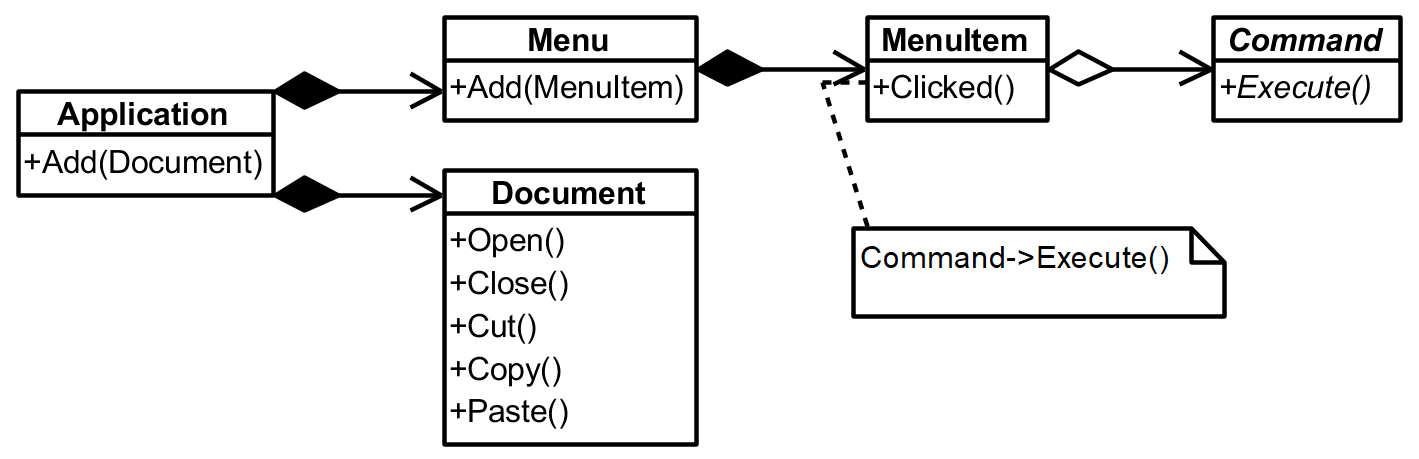
\includegraphics[width=0.9\textwidth]{commandExample.png}
        \end{center}
    \end{frame}

    \begin{frame}
        \frametitle{Команда вставки}
        \begin{center}
            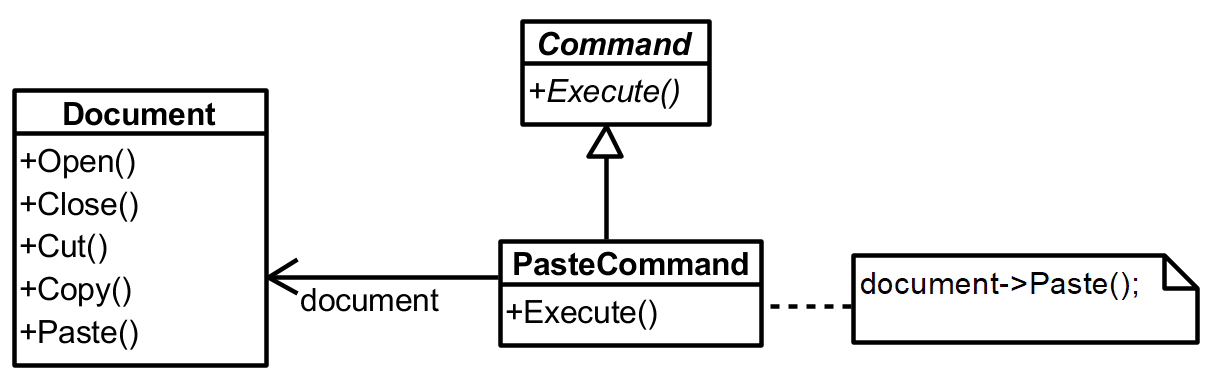
\includegraphics[width=0.75\textwidth]{pasteCommand.png}
        \end{center}
    \end{frame}

    \begin{frame}
        \frametitle{Команда открытия документа}
        \begin{center}
            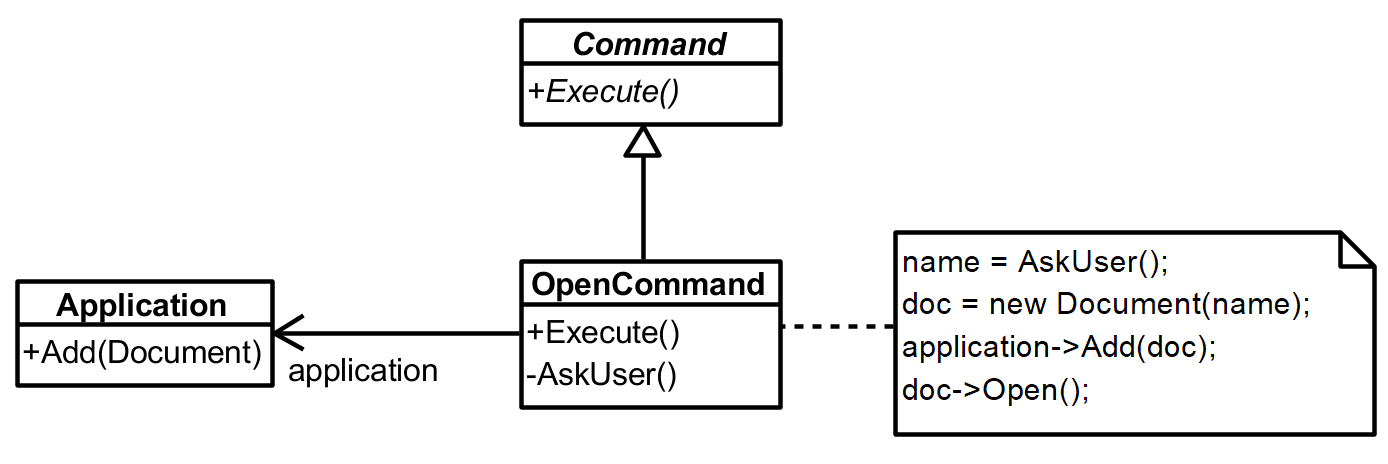
\includegraphics[width=0.75\textwidth]{openDocumentCommand.png}
        \end{center}
    \end{frame}

    \begin{frame}
        \frametitle{Составная команда}
        \begin{center}
            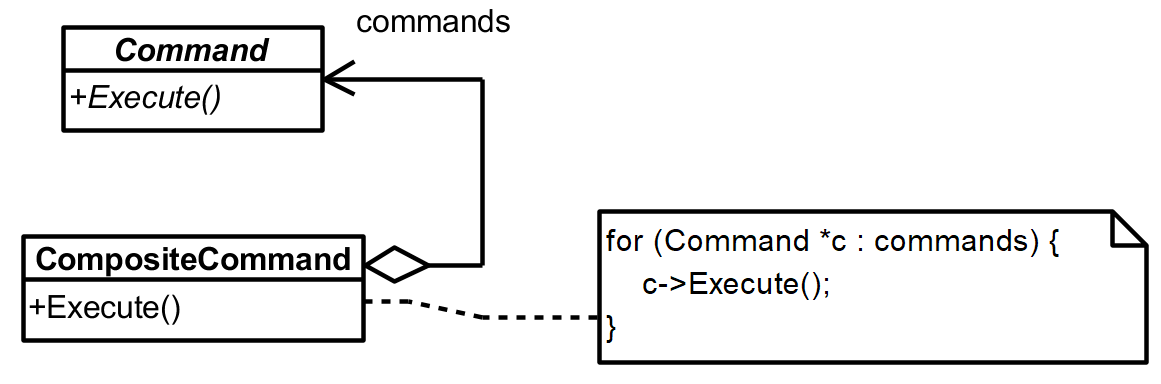
\includegraphics[width=0.75\textwidth]{compositeCommand.png}
        \end{center}
    \end{frame}

    \begin{frame}
        \frametitle{Паттерн ``Команда''}
        \begin{center}
            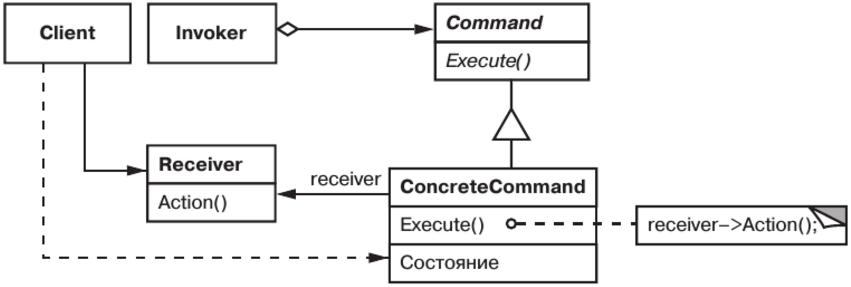
\includegraphics[width=0.9\textwidth]{command.png}
        \end{center}
    \end{frame}

    \begin{frame}
        \frametitle{Взаимодействие объектов}
        \begin{center}
            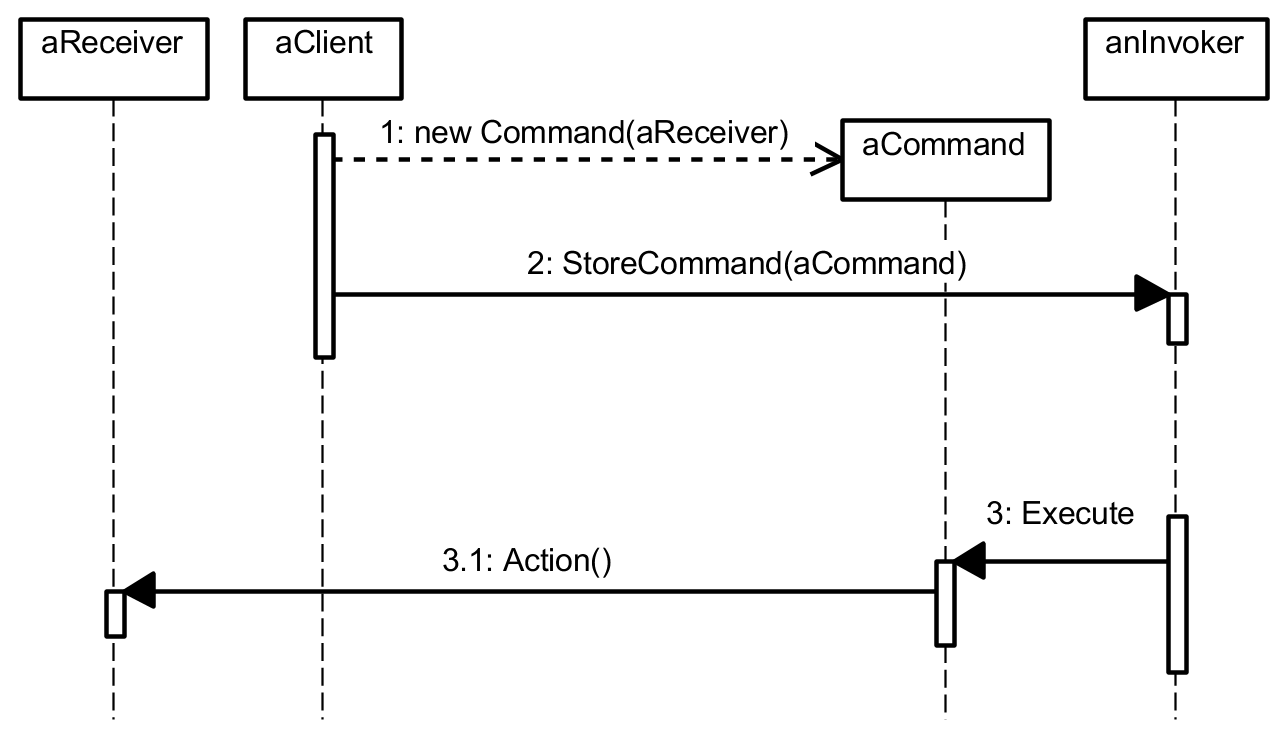
\includegraphics[width=0.9\textwidth]{commandSequence.png}
        \end{center}
    \end{frame}

    \begin{frame}
        \frametitle{Команда, применимость}
        \begin{itemize}
            \item Параметризовать объекты выполняемым действием
            \item Определять, ставить в очередь и выполнять запросы в разное время
            \item Поддержать отмену операций
            \item Структурировать систему на основе высокоуровневых операций, построенных из примитивных
            \item Поддержать протоколирование изменений
        \end{itemize}
    \end{frame}

    \begin{frame}
        \frametitle{``Команда'' (Command), детали реализации}
        \begin{itemize}
            \item Насколько ``умной'' должна быть команда
            \item Отмена и повторение операций --- тоже от хранения всего состояния в команде до ``вычислимого'' отката
            \begin{itemize}
                \item Undo-стек и Redo-стек
                \item Может потребоваться копировать команды
                \item ``Искусственные'' команды
                \item Композитные команды
            \end{itemize}
            \item Паттерн ``Хранитель'' для избежания ошибок восстановления
        \end{itemize}
    \end{frame}

    \begin{frame}[fragile]
        \frametitle{``Команда'', пример}
        \begin{itemize}
            \item Qt, класс QAction:
            \begin{minted}{c++}
const QIcon openIcon = QIcon(":/images/open.png");
QAction *openAct = new QAction(openIcon, tr("&Open..."), this);

openAct->setShortcuts(QKeySequence::Open);
openAct->setStatusTip(tr("Open an existing file"));

connect(openAct, &QAction::triggered, this, &MainWindow::open);

fileMenu->addAction(openAct);
fileToolBar->addAction(openAct);
            \end{minted}
        \end{itemize}
    \end{frame}

    \section{Паттерн ``Хранитель''}

    \begin{frame}
        \frametitle{Паттерн ``Хранитель'', мотивация}
        \begin{center}
            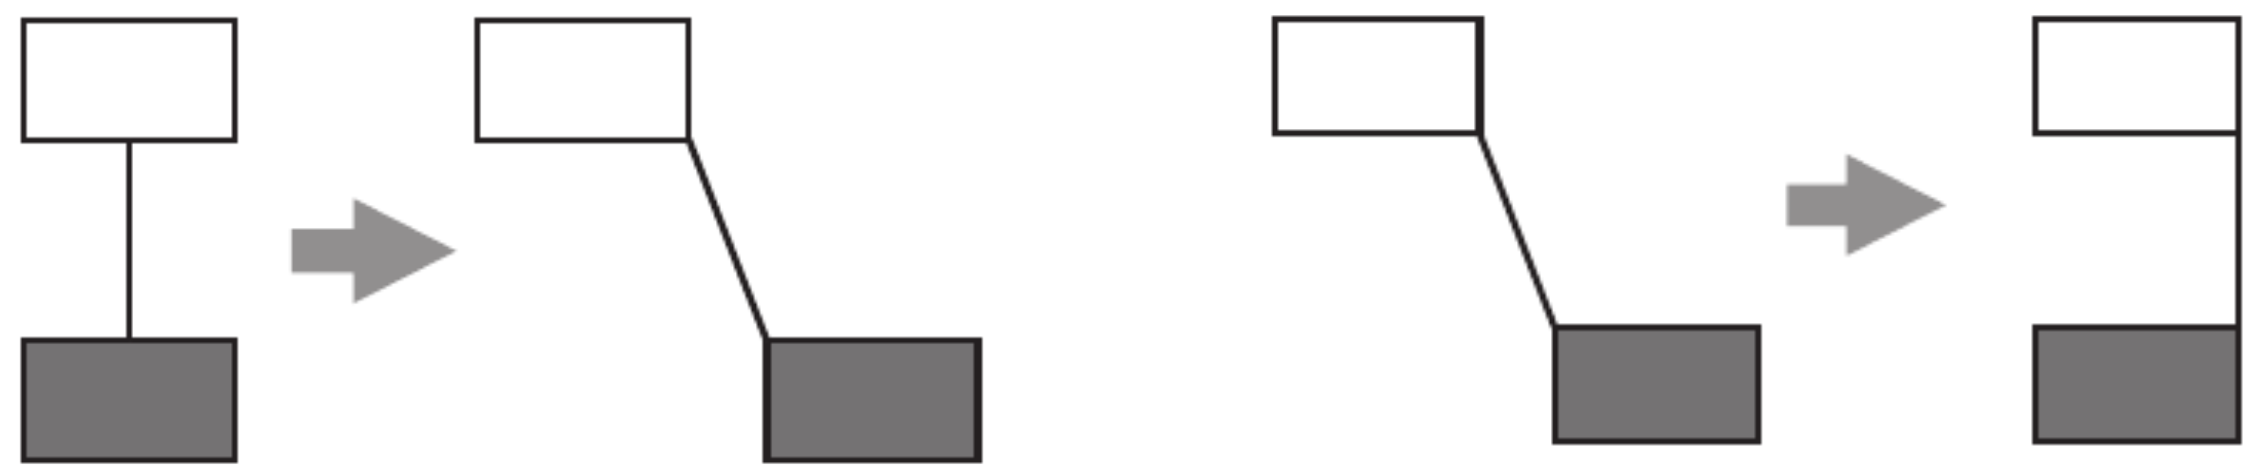
\includegraphics[width=0.9\textwidth]{mementoMotivation.png}
        \end{center}
        \begin{itemize}
            \item Хотим уметь фиксировать внутреннее состояние объектов
            \item И восстанавливать его при необходимости
            \item Не раскрывая внутреннего устройства объектов кому не надо
        \end{itemize}
    \end{frame}

    \begin{frame}
        \frametitle{Паттерн ``Хранитель''}
        \begin{center}
            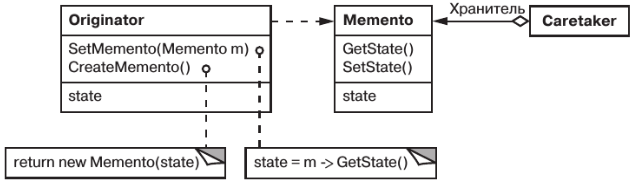
\includegraphics[width=0.7\textwidth]{memento.png}
        \end{center}
    \end{frame}

    \begin{frame}
        \frametitle{``Хранитель'' (Memento), детали реализации}
        \begin{itemize}
            \item Два интерфейса: ``широкий'' для хозяев и ``узкий'' для остальных объектов
            \begin{itemize}
                \item Требуется языковая поддержка
            \end{itemize}
            \item Можно хранить только дельты состояний
        \end{itemize}
    \end{frame}

    \section{Паттерн ``Состояние''}

    \begin{frame}
        \frametitle{Паттерн ``Состояние'', мотивация}
        \begin{center}
            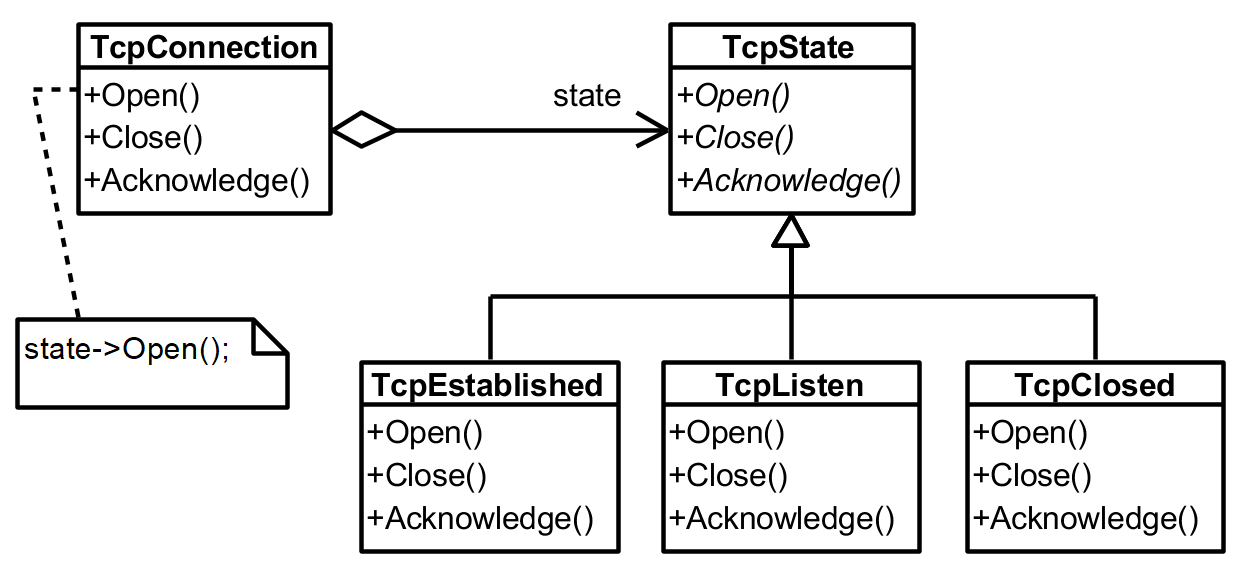
\includegraphics[width=0.85\textwidth]{stateExample.png}
        \end{center}
    \end{frame}

    \begin{frame}
        \frametitle{Паттерн ``Состояние''}
        \begin{center}
            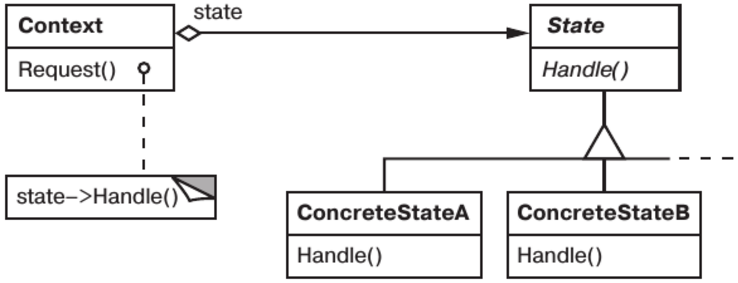
\includegraphics[width=0.75\textwidth]{state.png}
        \end{center}
    \end{frame}

    \begin{frame}
        \frametitle{``Состояние'' (State), детали реализации}
        \begin{itemize}
            \item Переходы между состояниями --- в Context или в State?
            \item Таблица переходов
            \begin{itemize}
                \item Трудно добавить действия по переходу
            \end{itemize}
            \item Создание и уничтожение состояний
            \begin{itemize}
                \item Создать раз и навсегда
                \item Создавать и удалять при переходах
            \end{itemize}
        \end{itemize}
    \end{frame}

    \begin{frame}
        \frametitle{``Состояние'' результаты}
        \begin{itemize}
            \item Локализует зависящее от состояния поведение
            \item Делает явными переходы между состояниями
            \item Объекты состояния можно разделять
        \end{itemize}
        Когда применять:
        \begin{itemize}
            \item Поведение объекта зависит от его состояния и должно изменяться во время выполнения
            \item Обилие условных операторов, в которых выбор ветви зависит от состояния
        \end{itemize}
    \end{frame}

    \section{Задача}

    \begin{frame}
        \frametitle{Задачи на остаток пары}
        Уточнить модель компьютерной игры Roguelike:

        \begin{enumerate}
            \item Используя шаблон ``Команда'' для поддержки взаимодействия с пользователем
            \item Используя паттерн ``Хранитель'' для поддержки сохранения/загрузки игры
            \item Используя паттерн ``Состояние'' для динамического переключения поведения мобов
            \begin{itemize}
                \item Мобы с низким здоровьем должны переключаться в трусливый режим
                \item По мере восстановления здоровья переходить в исходный
            \end{itemize}
        \end{enumerate}
    \end{frame}

\end{document}
